\documentclass{beamer}
\special{landscape}

%\usetheme{Berlin}
\usetheme{Warsaw}

%\usecolortheme{seahorse}
%\usefonttheme[onlysmall]{structurebold}

\setbeamertemplate{headline}[split]
\setbeamertemplate{footline}[default]
\setbeamertemplate{footline}[miniframes theme]
%\logo{\includegraphics[scale=0.25]{lifia_logo.png}}

\mode<presentation>
\usepackage[spanish]{babel}
\usepackage{beamerthemesplit}
\usepackage[utf8]{inputenc}
\usepackage{color}      % use if color is used in text


% Comandos en modo Verbatim
%\usepackage{fancyvrb}

\title{Practica 3 - Parte 3 - USART}
%\author{Juan Antonio Zubimendi\\azubimendi@lifia.info.unlp.edu.ar}

\AtBeginSection[]

\begin{document}

\begin{frame}
%\frametitle{Presentación}
\titlepage
\end{frame}

\section{USART - Introduccion}
\subsection{Introducción}
\begin{frame}
\frametitle{USART}
%\begin{block}{Slot Accounting System}
\begin{itemize}
 \item Convertidor paralelo-serie y serie-paralelo.
 \item Permite a la CPU comunicarse con dispositivos serie
 \item Posee tres registros, de 8 bits.
  \begin{itemize}
   \item DIN: Registro de entrada, recibir datos de la linea serie.
   \item DOUT: Registro de salida, escribir datos a enviar por linea serie.
   \item CTRL: Registro de Control (escritura) y estado (lectura).
  \end{itemize}
 \item La recepcion y envio de datos son independientes
 \item Los tres registros estan a partir de la posición 60h. 
  \begin{itemize}
      \item 60h = DIN
      \item 61h = DOUT
      \item 62h = CTRL
\end{itemize}
\end{itemize}
\end{frame}

\subsection{Interrupcion}
\begin{frame}
\frametitle{USART - Interrupciones}
%\begin{block}{Slot Accounting System}
\begin{itemize}
 \item La USART puede generar 2 interrupciones
  \begin{itemize}
   \item INT 2: Cuando hay un caracter para ser recibido.
   \item INT 3: Cuando esta listo para enviar un caracter.
  \end{itemize}
  \item En la practica no se va a considerar el uso de interrupciones
\end{itemize}
\end{frame}

\subsection{Caracteristicas de la Transmisión}
\begin{frame}
\frametitle{Caracteristicas}
%\begin{block}{Slot Accounting System}
\begin{itemize}
 \item Transmite 8bits por dato.
 \item Dos velocidades: V1: 6 baudios, V2: 18 baudios
 \item Comunicacion Sincrona o asincrona.
  \begin{itemize}
   \item Sincrona: 1 caracter de sincronismo, puede reconocer e insertar caracteres de sincronismo.
   \item Asincrono: Sin paridad, 1 bit de parada y 1 bit de arranque.
  \end{itemize}
 \item La recepcion y envio de datos son independientes
 \item Estas caracteristicas se configuran en el registro de control
\end{itemize}
\end{frame}

\subsection{Registro de Conrol}
\begin{frame}
\frametitle{Registro de Control}
%\begin{block}{Slot Accounting System}
\begin{center}
 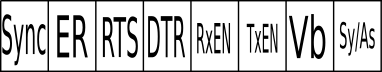
\includegraphics[scale=0.50]{usart-ctrl.png}
\end{center}

\begin{itemize}
 \item El registro de control 
 \begin{itemize}
   \item Sy/As: 0 = Sincrona / 1 = Asincrona
   \item Vb: Velocidad: 0 = 6 baudios/ 1 = 18 baudios
   \item TxEN: TxRDY 0 = inactivo / 1 = activo
   \item RxEN: RxRDY 0 = inactivo / 1 = activo
   \item DTR: Data Terminal Ready, 0 inactivo, 1 activo
   \item RTS: Request to Send, 0 inactivo, 1 activo
   \item ER: Error Reset, 1 = Resetea flags de errores
   \item Sync: 1 = Insercion y busqueda de caracteres de sincronismo (solo si Sy/AS = 0)
  \end{itemize}
\end{itemize}
\end{frame}

\begin{frame}
\frametitle{Registro de Estado}
%\begin{block}{Slot Accounting System}
\begin{center}
 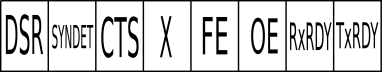
\includegraphics[scale=0.50]{usart-estado.png}
\end{center}
\begin{itemize}
 \item El registro de estado 
 \begin{itemize}
   \item DSR: Indica estado de linea DSR
   \item SYNDET: Si Sy/AS = 0, y Sync = 1, indica recepcion de caracter de sincronizacion
   \item CTS: Indica estado de entrada CTS
   \item FE: Indica error de recepcion, bits de parada incorrectos
   \item OE: 1 = Se recibio un caracter y todavia no se habia leido el anterior 
   \item RxRDY: 1 = El registro de entrada tiene un dato
   \item TxRDY: 1 = El registro salida esta vacio, listo
   \end{itemize}
\end{itemize}
\end{frame}

\subsection{Lineas de Datos de USART}
\begin{frame}[fragile]
\frametitle{Impresora Serie}
\begin{itemize}
 \item USART posee esta lineas
 \begin{itemize}
  \item rxd: Linea de salida, transmision serie 
  \item txd: Linea de entrada, recepcion serie
  \item dsr: Data Set Ready, el dispositivo conectado esta listo para recibir/ enviar datos
  \item rts: Request to Send, la USART quiere enviar datos
  \item cts: Clear To Send, el dispositivo esta listo para recibir datos
 \end{itemize}
\end{itemize}
\end{frame}

\section{Impresora Serie}
\subsection{Introduccion}
\begin{frame}[fragile]
\frametitle{Impresora Serie}
\begin{itemize}
 \item El simulador debe estar en la Configuración 4
 \item Utiliza una interfaz serie RS-232 simplificada
 \item Puede recibir hasta 5 caracteres
 \item Caracteristicas de Comunicacion
 \begin{itemize}
  \item Caracteres de 8 bits
  \item Dos velocidades (6 baudios y 18 baudios)
  \item Sin paridad
  \item Un bit de arranque (0)
  \item Un bit de parada (1)
 \end{itemize}
  \item Dos protocolos de Comunicacion
\begin{itemize}
 \item Software XON/XOFF
 \item Hardware DTR
\end{itemize}

\end{itemize}
\end{frame}


\subsection{Introduccion}
\begin{frame}[fragile]
\frametitle{Conexion USART - Impresora Serie}
\begin{itemize}
 \item La conexion USART e Impresora usa las siguientes lineas:
 \begin{itemize}
  \item TxD: Linea de Transmisión serie, la CPU transmite los datos a imprimir
  \item RxD: Linea de recepcion serie, los datos enviados desde la impresora a la CPU
  \item DTR: Linea de salida que habilita/inhabilita la transmision de datos a la impresora
\end{itemize}
\item Las lineas de RTS y CTS de la USART estan conectadas entre si (no interviene la impresora)
\end{itemize}
\end{frame}

\section{Protocolos de Comunicacion}
\subsection{Software XON/XOFF}
\begin{frame}[fragile]
\frametitle{XON/XOFF}
\begin{itemize}
 \item Configurar la impresora para usar el protocolo DTR usando el comado `` pi x''
 \item Utiliza unicamente TxD y RxD.
 \item Cuando el buffer de recepecion esta lleno, la impresora envia el caracter XOFF a traves de la linea TxD, para detener la transmision de datos
 \item Cuando hay espacio en el buffer, la impresora envia el caracter XON, avisando que se puede seguir enviando caracteres
 \item El Caracter XOFF es 13h
 \item El Caracter XON es 11h
 \item Puede ser mediante Interrupciones o consulta de estado
\end{itemize}

\end{frame}

\subsection{Hardware DTR}
\begin{frame}[fragile]
\frametitle{DTR}
\begin{itemize}
 \item Configurar la impresora para usar el protocolo DTR usando el comado `` pi d'' 
 \item La linea DTR indica si se debe iniciar/suspender la transmision de datos.
 \item Si el buffer esta lleno, la impresora pone 0 en la linea DTR.
 \item Si el buffer tiene lugar, la impresora pone 1 en la linea DTR.
 \item Puede ser mediante Interrupciones o consulta de estado
\end{itemize}

\end{frame}


\section{Uso por Consulta de Estado}

\subsection{Protocolo XON-XOFF}

\begin{frame}[fragile]
\frametitle{Como configurar la Impresora con XON/XOFF}
\begin{itemize}
 \item El simulador debe estar en la configuración 4
 \item Se configura la USART con el numero 51H (en binario 01010001 en el registro de control.
 \begin{itemize}
 \item Error reset activo (bit 6)
 \item DTR activado (bit 4)
 \item Comunicacion asincrona (bit 0). 
\end{itemize}

 \end{itemize}
\end{frame}

\begin{frame}[fragile]
\frametitle{Como usar la Impresora con XON/XOFF}

\begin{itemize}
\item Esperamos a que la USART este lista para enviar un caracter. 
\begin{itemize}
\item Es decir TxRDY cambia a 1 
\end{itemize}
\item Enviamos el caracter a imprimir. 
\item Verificar si recibimos un caracter
\begin{itemize}
 \item Es decir RxRDY cambia a 1
\end{itemize}
\item Si no recibimos un caracter, podemos enviar el siguiente caracter
\item Si recibimos un caracter, puede ser XON o XOFF
\begin{itemize}
\item Si recibimos XON, podemos seguir imprimiendo.
\item Si recibimos XOFF, hay que esperar hasta recibir XON para poder imprimir.
\end{itemize}
\end{itemize}

\end{frame}


\subsection{Protocolo DTR}
\begin{frame}[fragile]
\frametitle{Como configurar la Impresora con DTR}
\begin{itemize}
 \item El simulador debe estar en la configuración 4
 \item Se configura la USART con el numero binario 01010001
 \begin{itemize}
 \item Error reset (bit 6 en 1)
 \item DTR activado (bit 4 en 1)
 \item Comunicacioón asincrona (bit 0 en 1)
\end{itemize}
\end{itemize}

\end{frame}


\begin{frame}[fragile]
\frametitle{Como usar la Impresora con DTR}
\begin{itemize}
 \item  Consultamos para saber si esta lista para recibir un caracter. Se deben dar estas condiciones:
 \begin{itemize}
  \item Data Set Ready = 1, la impresora debe estar lista para recibir caracter (bit de estado 7)
  \item TxRDY = 1, la USART debe estar lista para transmitir (bit de estado 0) 
 \end{itemize}
\item Transmitimos el siguiente caracter 
\item Volvemos a empezar si nos quedan mas caracteres a enviar a la impresora.
\end{itemize}

\end{frame}

\end{document}

